\documentclass[conference]{IEEEtran}
\IEEEoverridecommandlockouts
% The preceding line is only needed to identify funding in the first footnote. If that is unneeded, please comment it out.
\usepackage{cite}
\usepackage{amsmath,amssymb,amsfonts}
\usepackage{algorithmic}
\usepackage{graphicx}
\usepackage{textcomp}
\usepackage{xcolor}
\usepackage{tabularx}
\usepackage{multirow}
\usepackage{graphics} % for pdf, bitmapped graphics files
\usepackage{subfig}
\usepackage{subcaption}
\usepackage{hyperref}
\usepackage{academicons}
\usepackage{xcolor}
\def\BibTeX{{\rm B\kern-.05em{\sc i\kern-.025em b}\kern-.08em
		T\kern-.1667em\lower.7ex\hbox{E}\kern-.125emX}}
% Gráficas en MATLAB
\usepackage{tikz, pgfplots}
\usepackage{listings}
% Control 
\usepackage{amsmath}
% Color Enlace
\definecolor{colorEnlace}{RGB}{0, 0, 0}
\hypersetup{
	colorlinks=true,
	linkcolor=colorEnlace,
	citecolor=colorEnlace,
	urlcolor=colorEnlace,
	pdfauthor={Davis Bremdow Salazar Roa},
	pdftitle={Introducción a LaTeX}
}
% Configuración del listing
\lstdefinelanguage{VHDL}{
	morekeywords={
		library, use, all, entity, is, port, in, out, architecture, of, begin, end, process, if, then, else, elsif, when, others,
		signal, variable, constant, wait, for, generate, with, select, after, report, severity
	},
	sensitive=true,
	morecomment=[l]--,      % Comentarios de una sola línea
	morestring=[b]"        % Cadenas entre comillas dobles
}

\lstset{
	language=VHDL,
	basicstyle=\ttfamily\small,      % Estilo básico del texto
	keywordstyle=\color{blue}\bfseries, % Color para palabras clave
	commentstyle=\color{green!60!black}, % Color para comentarios
	stringstyle=\color{red},        % Color para cadenas
	numbers=left,                   % Números de línea a la izquierda
	numberstyle=\tiny\color{gray},  % Estilo de los números de línea
	stepnumber=1,                   % Incremento entre los números de línea
	breaklines=true,                % Saltar líneas largas
	frame=single,                   % Marco alrededor del código
	captionpos=b,                   % Posición del título (b=abajo)
	tabsize=1,                      % Tamaño de tabulación
}

\begin{document}
	
	\title{Aplicaciones digitales en VHDL}
	\author{	
		\IEEEauthorblockN{Davis Bremdow Salazar Roa}
		\IEEEauthorblockA{Universidad Nacional de San Antonio Abad del Cusco}
		\textit{Escuela Profesional de Ingeniería Electrónica}\\
		\textit{Arquitectura de Microcontroladores y Microprocesadores}\\
		200353 \\\\
		Cusco, Perú
	}
	\maketitle
	
	\begin{abstract}
	Programming gates, adders, comparators, and registers in VHDL involves modeling fundamental digital components for various applications. Logic gates such as AND, OR, and XOR are the building blocks, implemented using simple concurrent assignments or processes. Adders, including half-adders and full-adders, are designed to perform binary addition, often leveraging gates and constructs like the with-select statement or nested conditional statements for clarity and scalability.
	
	Comparators evaluate binary inputs to determine equality, magnitude, or other relationships. They are typically implemented using conditional or concurrent assignments to evaluate logical conditions. Registers, essential for sequential circuits, store data and are commonly built using flip-flops or processes triggered by clock signals, ensuring synchronization. Together, these components illustrate the versatility of VHDL in designing both combinational and sequential circuits, enabling the creation of reliable and scalable digital systems.
	\end{abstract}
	
	\begin{IEEEkeywords}
		Compilador, Generador de Léxico, Generador Sintáctico, Generador Sintáctico
	\end{IEEEkeywords}
	
	\section{Introducción}
	VHDL (VHSIC Hardware Description Language) es un lenguaje de descripción de hardware ampliamente utilizado para modelar y simular sistemas digitales. Diseñado inicialmente para respaldar el desarrollo de circuitos electrónicos complejos, permite describir el comportamiento y la estructura de hardware a nivel lógico y físico. Con su sintaxis similar a los lenguajes de programación tradicionales, VHDL facilita la creación de diseños modulares y reutilizables, adaptándose tanto al modelado conceptual como a la implementación final en dispositivos como FPGAs y ASICs.
	
	A diferencia de los lenguajes de programación comunes, VHDL se enfoca en la concurrencia, permitiendo definir múltiples procesos que se ejecutan simultáneamente. Esto lo hace ideal para sistemas digitales donde las señales y los eventos temporales son cruciales. Gracias a su capacidad para simular diseños antes de su implementación física, VHDL es una herramienta esencial en el desarrollo de hardware fiable y eficiente.
	
	% // ==================== EJERCICIO 01 ============================ //
	\section{Puerta Lógica AND de 8 bits}
	\subsection{Código}
	
	\begin{lstlisting}[numbers=none]
		 library ieee;
		use ieee.std_logic_1164.all;
		
		
		entity andgate8bits is
		port(
		A, B: in std_logic_vector(7 downto 0);
		C : out std_logic_vector(7 downto 0)
		);
		end entity;
		
		architecture arch of andgate8bits is
		begin
		C <= A and B;
		end;
	\end{lstlisting}
	
	\subsection{Simulación}
	\begin{figure}[h]
		\centering
		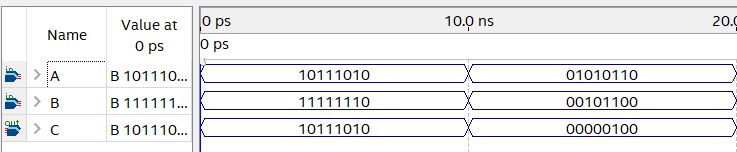
\includegraphics[width=0.5\textwidth]{media/andgate8bits}
		\caption{Simulación compuerta And 8 bits - Forma de Onda}
		\label{fig:andgate8bits}
	\end{figure}
	
	% // ==================== EJERCICIO 02 ============================ //
	\section{Puerta OR de 8 bits}
	\subsection{Código}
	\begin{lstlisting}[numbers=none]
		 library ieee;
		use ieee.std_logic_1164.all;
		
		
		entity orgate8bits is
		port(
		A, B: in std_logic_vector(7 downto 0);
		C : out std_logic_vector(7 downto 0)
		);
		end entity;
		
		architecture arch of orgate8bits is
		begin
		C <= A or B;
		end;
	\end{lstlisting}
	\subsection{Simulación}
	\begin{figure}[h]
		\centering
		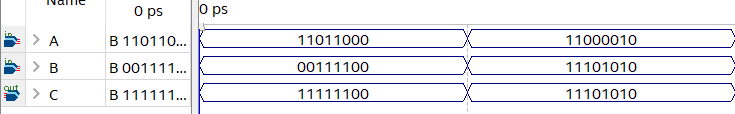
\includegraphics[width=0.5\textwidth]{media/orgate8bits}
		\caption{Simulación compuerta OR 8 de bits - Forma de Onda}
		\label{fig:orgate8bits1}
	\end{figure}
	
	% // ==================== EJERCICIO 03 ============================ //
	\section{Inversor de 8 bits (NOT)}
	\subsection{Código}
	\begin{lstlisting}[numbers=none]
		 library ieee;
		use ieee.std_logic_1164.all;
		
		
		entity notgate8bits is
		port(
		A : in std_logic_vector(7 downto 0);
		B : out std_logic_vector(7 downto 0)
		);
		end entity;
		
		architecture arch of notgate8bits is
		begin
		B <= not A;
		end;s
	\end{lstlisting}
	\subsection{Simulación}
	\begin{figure}[h]
		\centering
		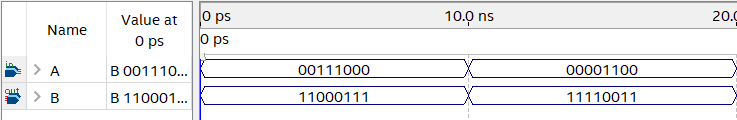
\includegraphics[width=0.5\textwidth]{media/notgate8bits1}
		\caption{Simulación compuerta NOT 8 bits - forma de onda}
		\label{fig:notgate8bits1}
	\end{figure}
	
	
	% // ==================== EJERCICIO 04 ============================ //
	\section{Sumador de 8 bits sin acarreo}
	\subsection{Código}
	\begin{lstlisting}[numbers=none]
		library IEEE;
		use IEEE.STD_LOGIC_1164.ALL;
		use IEEE.STD_LOGIC_ARITH.ALL;
		use IEEE.STD_LOGIC_UNSIGNED.ALL;
		
		entity sumador8bits is
		Port (
		A : in STD_LOGIC_VECTOR (7 downto 0);
		B : in STD_LOGIC_VECTOR (7 downto 0);
		SUM : out STD_LOGIC_VECTOR (7 downto 0)
		);
		end entity;
		
		architecture Behavioral of sumador8bits is
		begin
		process(A, B)
		begin
		SUM <= A + B;
		end process;
		end architecture;
		
	\end{lstlisting}
	\subsection{Simulación}
	\begin{figure}[h]
		\centering
		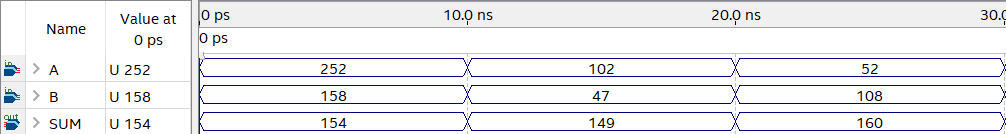
\includegraphics[width=0.5\textwidth]{media/sumador8bits}
		\caption{Simulación Sumador 8 bits -forma de onda}
		\label{fig:sumador8bits}
	\end{figure}
	
	Como se puede ver la figura \ref{fig:sumador8bits} el resultado de la primera columna es erroneo, esto debido a que existe un desbordamiento en la suma y el resultado que para los propósitos solicitados solo es de 8 bits, por lo que para obtener un resultado adecuado, es necesario agregar un bit de acarreo o en su defecto el resultado de la suma debe ser de 9 bits.
	
	% // ==================== EJERCICIO 05 ============================ //
	\section{Restador de 8 bits con indicador de desbordamiento}
	\subsection{Código}
	\begin{lstlisting}[numbers=none]
		library IEEE;
		use IEEE.STD_LOGIC_1164.ALL;
		use IEEE.STD_LOGIC_ARITH.ALL;
		use IEEE.STD_LOGIC_UNSIGNED.ALL;
		
		entity restador8Bits is
		Port (
		A : in std_logic_vector (7 downto 0);
		B : in std_logic_vector (7 downto 0);
		diferencia : out std_logic_vector (7 downto 0);
		desbordamiento : out std_logic
		);
		end entity;
		
		architecture Behavioral of restador8Bits is
		signal tempA : std_logic_vector (8 downto 0);
		signal tempB : std_logic_vector (8 downto 0);
		signal resta_temporal : std_logic_vector (8 downto 0);
		begin
		process(A, B)
		begin
		tempA <= '0' & A; -- Extender A a 9 bits
		tempB <= '0' & B; -- Extender B a 9 bits
		
		resta_temporal <= tempB - tempA;
		
		diferencia <= resta_temporal(7 downto 0); -- Resultado de 8 bits
		
		-- Verificar desbordamiento
		if (A(7) = '0' and B(7) = '1' and resta_temporal(8) = '1') or
		(A(7) = '1' and B(7) = '0' and resta_temporal(8) = '0') then
		desbordamiento <= '1';
		else
		desbordamiento <= '0';
		end if;
		end process;
		end architecture;
		
	\end{lstlisting}
	\subsection{Simulación}
	\begin{figure}[h]
		\centering
		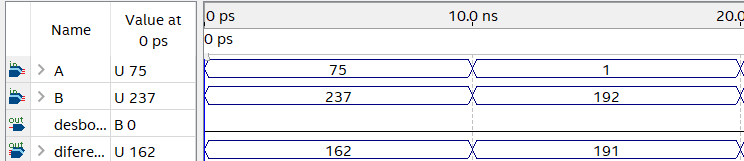
\includegraphics[width=0.5\textwidth]{media/restador8bits}
		\caption{Simulación restador 8 bits - forma de onda}
		\label{fig:restador8bits}
	\end{figure}

	% // ==================== EJERCICIO 06 ============================ //
	\section{Multiplicador de 8 bits con control de habilitación y señal de fin de operación}
	\subsection{Código}
	\begin{lstlisting}[numbers=none]
		library IEEE;
		use IEEE.STD_LOGIC_1164.ALL;
		use IEEE.STD_LOGIC_ARITH.ALL;
		use IEEE.STD_LOGIC_UNSIGNED.ALL;
		
		entity multiplicador8bits is
		Port (
		A, B : in std_logic_vector (7 downto 0);
		en : in std_logic;
		final : out std_logic;
		producto : out std_logic_vector (15 downto 0)
		);
		end entity;
		
		architecture Behavioral of multiplicador8bits is
		begin
		process(A, B)
		begin
		if en = '1' then
		producto <= A * B;
		final <= '1';
		else
		final <= '0';
		producto <= (others => '0');
		end if;
		end process;
		end architecture;
		
	\end{lstlisting}
	\subsection{Simulación}
	\begin{figure}[h]
		\centering
		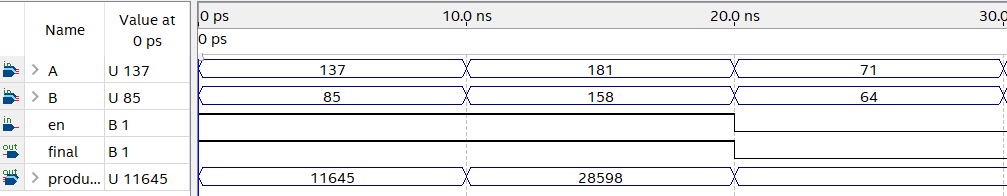
\includegraphics[width=0.5\textwidth]{media/multiplicador8bits}
		\caption{Simulación multiplicador 8 bits - forma de onda}
		\label{fig:multiplicador8bits}
	\end{figure}
	
	% // ==================== EJERCICIO 07 ============================ //
	\section{Divisor de 8 bits con cálculo de cociente y residuo}
	\subsection{Código}
	\begin{lstlisting}[numbers=none]
		library IEEE;
		use IEEE.STD_LOGIC_1164.ALL;
		use IEEE.NUMERIC_STD.ALL;
		
		entity divisor8Bits is
		Port (
		A : in std_logic_vector (7 downto 0); -- Dividendo
		B : in std_logic_vector (7 downto 0); -- Divisor
		cociente : out std_logic_vector (7 downto 0);
		residuo : out std_logic_vector (7 downto 0)
		);
		end entity;
		
		architecture Behavioral of divisor8Bits is
		signal temp_cociente : unsigned (7 downto 0);
		signal temp_residuo : unsigned (7 downto 0);
		signal tempA :  unsigned (7 downto 0);
		signal tempB : unsigned (7 downto 0);
		begin
		process(A, B)
		begin
		tempA <= unsigned(A);
		tempB <= unsigned(B);
		
		-- Verifica que no se realice una division por cero
		if tempB /= 0 then
		temp_cociente <= tempA / tempB;
		temp_residuo <= tempA mod tempB;
		else
		temp_cociente <= (others => '0');
		temp_residuo <= (others => '0');
		end if;
		end process;
		
		cociente <= std_logic_vector(temp_cociente);
		residuo <= std_logic_vector(temp_residuo);
		end architecture;
	\end{lstlisting}
	\subsection{Simulación}
	\begin{figure}[h]
		\centering
		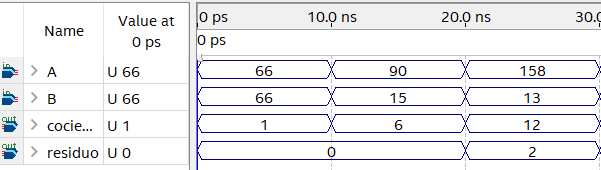
\includegraphics[width=0.5\textwidth]{media/divisor8bits}
		\caption{Simulación Divisor 8 bits -Forma de Onda}
		\label{fig:divisor8bits}
	\end{figure}
	
	% // ==================== EJERCICIO 08 ============================ //
	\section{Comparador de 8 bits con registros de bandera (flags)}
	\subsection{Código}
	\begin{lstlisting}[numbers=none]
		library IEEE;
		use IEEE.STD_LOGIC_1164.ALL;
		use IEEE.STD_LOGIC_ARITH.ALL;
		use IEEE.STD_LOGIC_UNSIGNED.ALL;
		
		entity comparador8Bits is
		Port (
		A, B : in STD_LOGIC_VECTOR (7 downto 0);
		igual, Amayor, Amenor: out std_logic
		);
		end entity;
		
		architecture Behavioral of comparador8Bits is
		begin
		process(A, B)
		begin
		if A = B then
		igual <= '1';
		Amayor <= '0';
		Amenor <= '0';
		elsif A < B then
		igual <= '0';
		Amenor <= '1';
		Amayor <= '0';
		else
		igual <= '0';
		Amenor <= '0';
		Amayor <= '1';
		end if;
		end process;
		end architecture;
		
	\end{lstlisting}
	\subsection{Simulación}
	\begin{figure}[h]
		\centering
		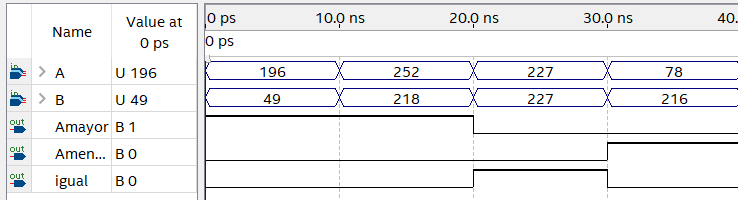
\includegraphics[width=0.5\textwidth]{media/comparador8bits}
		\caption{Simulación comparador 8 bits - forma de onda}
		\label{fig:comparador8bits}
	\end{figure}
	
	% // ==================== EJERCICIO 09 ============================ //
	\section{Registro de 8 bits con habilitación de carga y reset asíncrono}
	\subsection{Código}
	\begin{lstlisting}[numbers=none]
		library IEEE;
		use IEEE.STD_LOGIC_1164.ALL;
		
		entity registro8Bits is
		Port (
		clk : in STD_LOGIC;
		en, reset : in STD_LOGIC;
		data_in : in STD_LOGIC_VECTOR (7 downto 0);
		data_out : out STD_LOGIC_VECTOR (7 downto 0)
		);
		end entity ;
		
		architecture Behavioral of registro8Bits is
		signal reg_data : STD_LOGIC_VECTOR (7 downto 0);
		begin
		process(clk, reset)
		begin
		if en = '1' then
		
		if reset = '1' then
		reg_data <= (others => '0');
		elsif rising_edge(clk) then
		reg_data <= data_in;
		end if;
		
		else
		reg_data <= (others => '0');
		end if;
		end process;
		data_out <= reg_data;
		end architecture;
	\end{lstlisting}
	\subsection{Simulación}
	\begin{figure}[h]
		\centering
		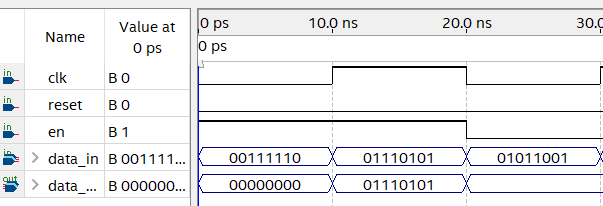
\includegraphics[width=0.5\textwidth]{media/registro8bit}
		\caption{Simulación Registro 8 bits - Forma de Onda}
		\label{fig:registro8bit}
	\end{figure}
	
	% // ==================== EJERCICIO 10 ============================ //
	\section{Registro de desplazamiento de 8 bits con habilitación de desplazamiento, dirección y entrada de datos en serie}
	\subsection{Código}
	\begin{lstlisting}[numbers=none]
		library IEEE;
		use IEEE.STD_LOGIC_1164.ALL;
		use IEEE.STD_LOGIC_ARITH.ALL;
		use IEEE.STD_LOGIC_UNSIGNED.ALL;
		
		entity desplazamiento8bits is
		Port (
		clk : in std_logic;
		en, reset : in std_logic;
		data_in : in std_logic_vector(7 downto 0);
		shift_in : in std_logic;
		data_out : out std_logic_vector (7 downto 0)
		);
		end entity;
		
		architecture Behavioral of desplazamiento8bits is
		signal reg_data : std_logic_vector (7 downto 0);
		begin
		process(en, clk, reset)
		begin
		if en = '1' then
		if reset = '1' then
		reg_data <= (others => '0');
		elsif rising_edge(clk) then
		reg_data <= data_in;
		reg_data <= shift_in & data_in(7 downto 1);
		end if;
		else
		reg_data <= (others => '0');
		end if;
		end process;
		data_out <= reg_data;
		end architecture;
	\end{lstlisting}
	\subsection{Simulación}
	\begin{figure}[h]
		\centering
		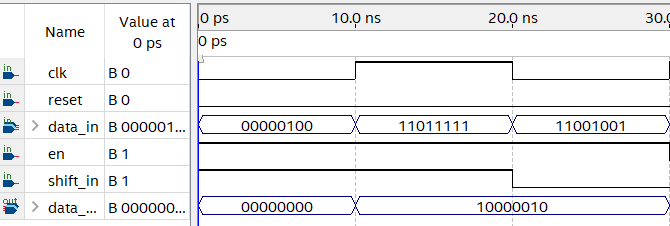
\includegraphics[width=0.5\textwidth]{media/desplazamiento8bits}
		\caption{Simulación desplazamiento 8 bits - forma de onda}
		\label{fig:desplazamiento8bits}
	\end{figure}
	
	\bibliographystyle{IEEEtran}
	\bibliography{biblio}
\end{document}

